\documentclass[25pt, a0papper, portrait]{tikzposter}
\usepackage[utf8]{inputenc}
\usepackage{xcolor}
\usepackage{graphicx,mwe}
\usepackage{filecontents}% http://ctan.org/pkg/filecontents
\usepackage{lipsum}% http://ctan.org/pkg/lipsum
\usepackage{tikz}
\usepackage{multicol}
\usepackage{adjustbox}

\makeatletter
\def\TP@titlegraphictotitledistance{-9cm}
\settitle{ \centering \vbox{
		\@titlegraphic \\ [\TP@titlegraphictotitledistance] 
		\centering
		\color{titlefgcolor} {\bfseries \Huge \sc \@title \par}
		\vspace*{1em}
		{\huge \@author \par} \vspace*{1em} {\LARGE \@institute}
	}}
\makeatother
 
\title{TCPSnitch: Dissecting the Socket API Usage}
\author{\textbf{Gregory Vander Schueren}, Quentin De Coninck, Olivier Bonaventure \\ \texttt{gregory.vanderschueren@tessares.net} \\ \texttt{https://tcpsnitch.org}}
\date{\today}
\titlegraphic{
	
\includegraphics[width=0.06\textwidth]{figures/UCL}
    \hfill

\includegraphics[width=0.15\textwidth]{figures/tessares}
}

\institute{Université catholique de Louvain, Louvain-la-Neuve, Belgium}
 
\usepackage{blindtext}
\usepackage{comment}
\renewcommand*\familydefault{\sfdefault}
\usepackage[T1]{fontenc}
 
\usetheme{Desert}
\usenotestyle{Sticky}

\usepackage[backend=bibtex]{biblatex}
\addbibresource{biblio.bib,2011.bib}

\tikzposterlatexaffectionproofoff
\begin{document}
\maketitle

%{%<--------- Start scope
	\colorlet{notebgcolor}{yellow} %<---- change color
	%\block{BlocktitleB}{\lipsum[2]}
%}%<--------- End scope

% FIRST ROW
\begin{columns}
    \column{0.50}
    \block{TCPSnitch}{
        \begin{itemize}
            \item Software that collects detailed traces of the
                  interactions between networked applications and the TCP/IP stack.
            \item Tracks the functions that are applied on each socket with
                their timestamp, parameters, return value, thread id, etc.
            \item Able to trace sequence of calls and allows to
                detect patterns of interactions.
            \item Runs on both Linux and Android.
        \end{itemize}
        \vspace{0.8cm}
        TCPSnitch runs the specified command until it exits, much like tcpdump:
        \begin{tikzfigure}
            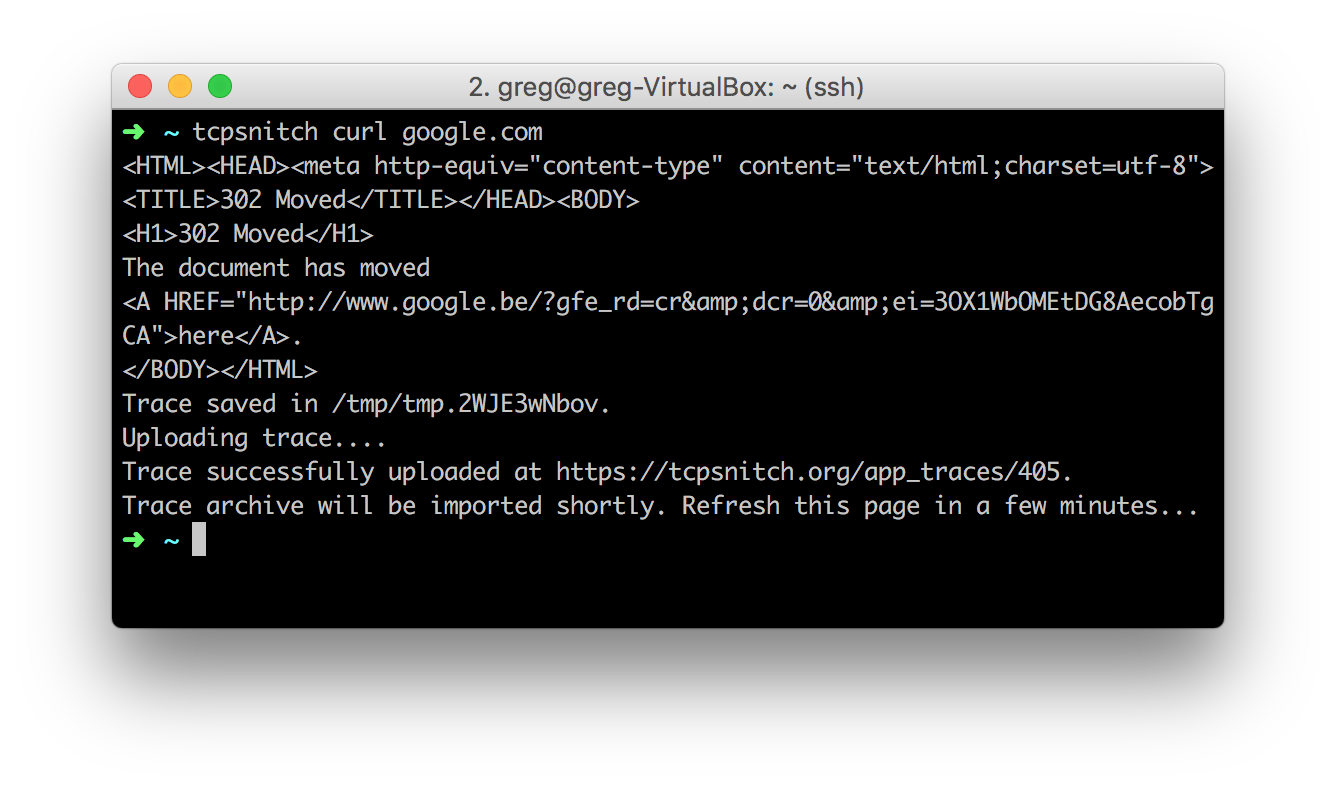
\includegraphics[width=.4\textwidth]{figures/tcpsnitch}
        \end{tikzfigure}
        TCPSnitch is open-source: \url{https://github.com/GregoryVds/tcpsnitch}.
    }
    \column{0.50}
    \block{Public dataset: \url{https://tcpsnitch.org}}{
        \begin{itemize}
            \item TCPSnitch automatically uploads traces to \url{https://tcpsnitch.org}.
            \item Public platform designed to centralize and visualize the traces.
            \item Currently contains traces for more than 130 applications on Linux and Android.
            \item In total, this represents about 5 M function calls on 25 K sockets.
        \end{itemize}
        \vspace{0.8cm}
        Upon uploading a trace, multiple metrics and charts are computed:
        \begin{tikzfigure}
            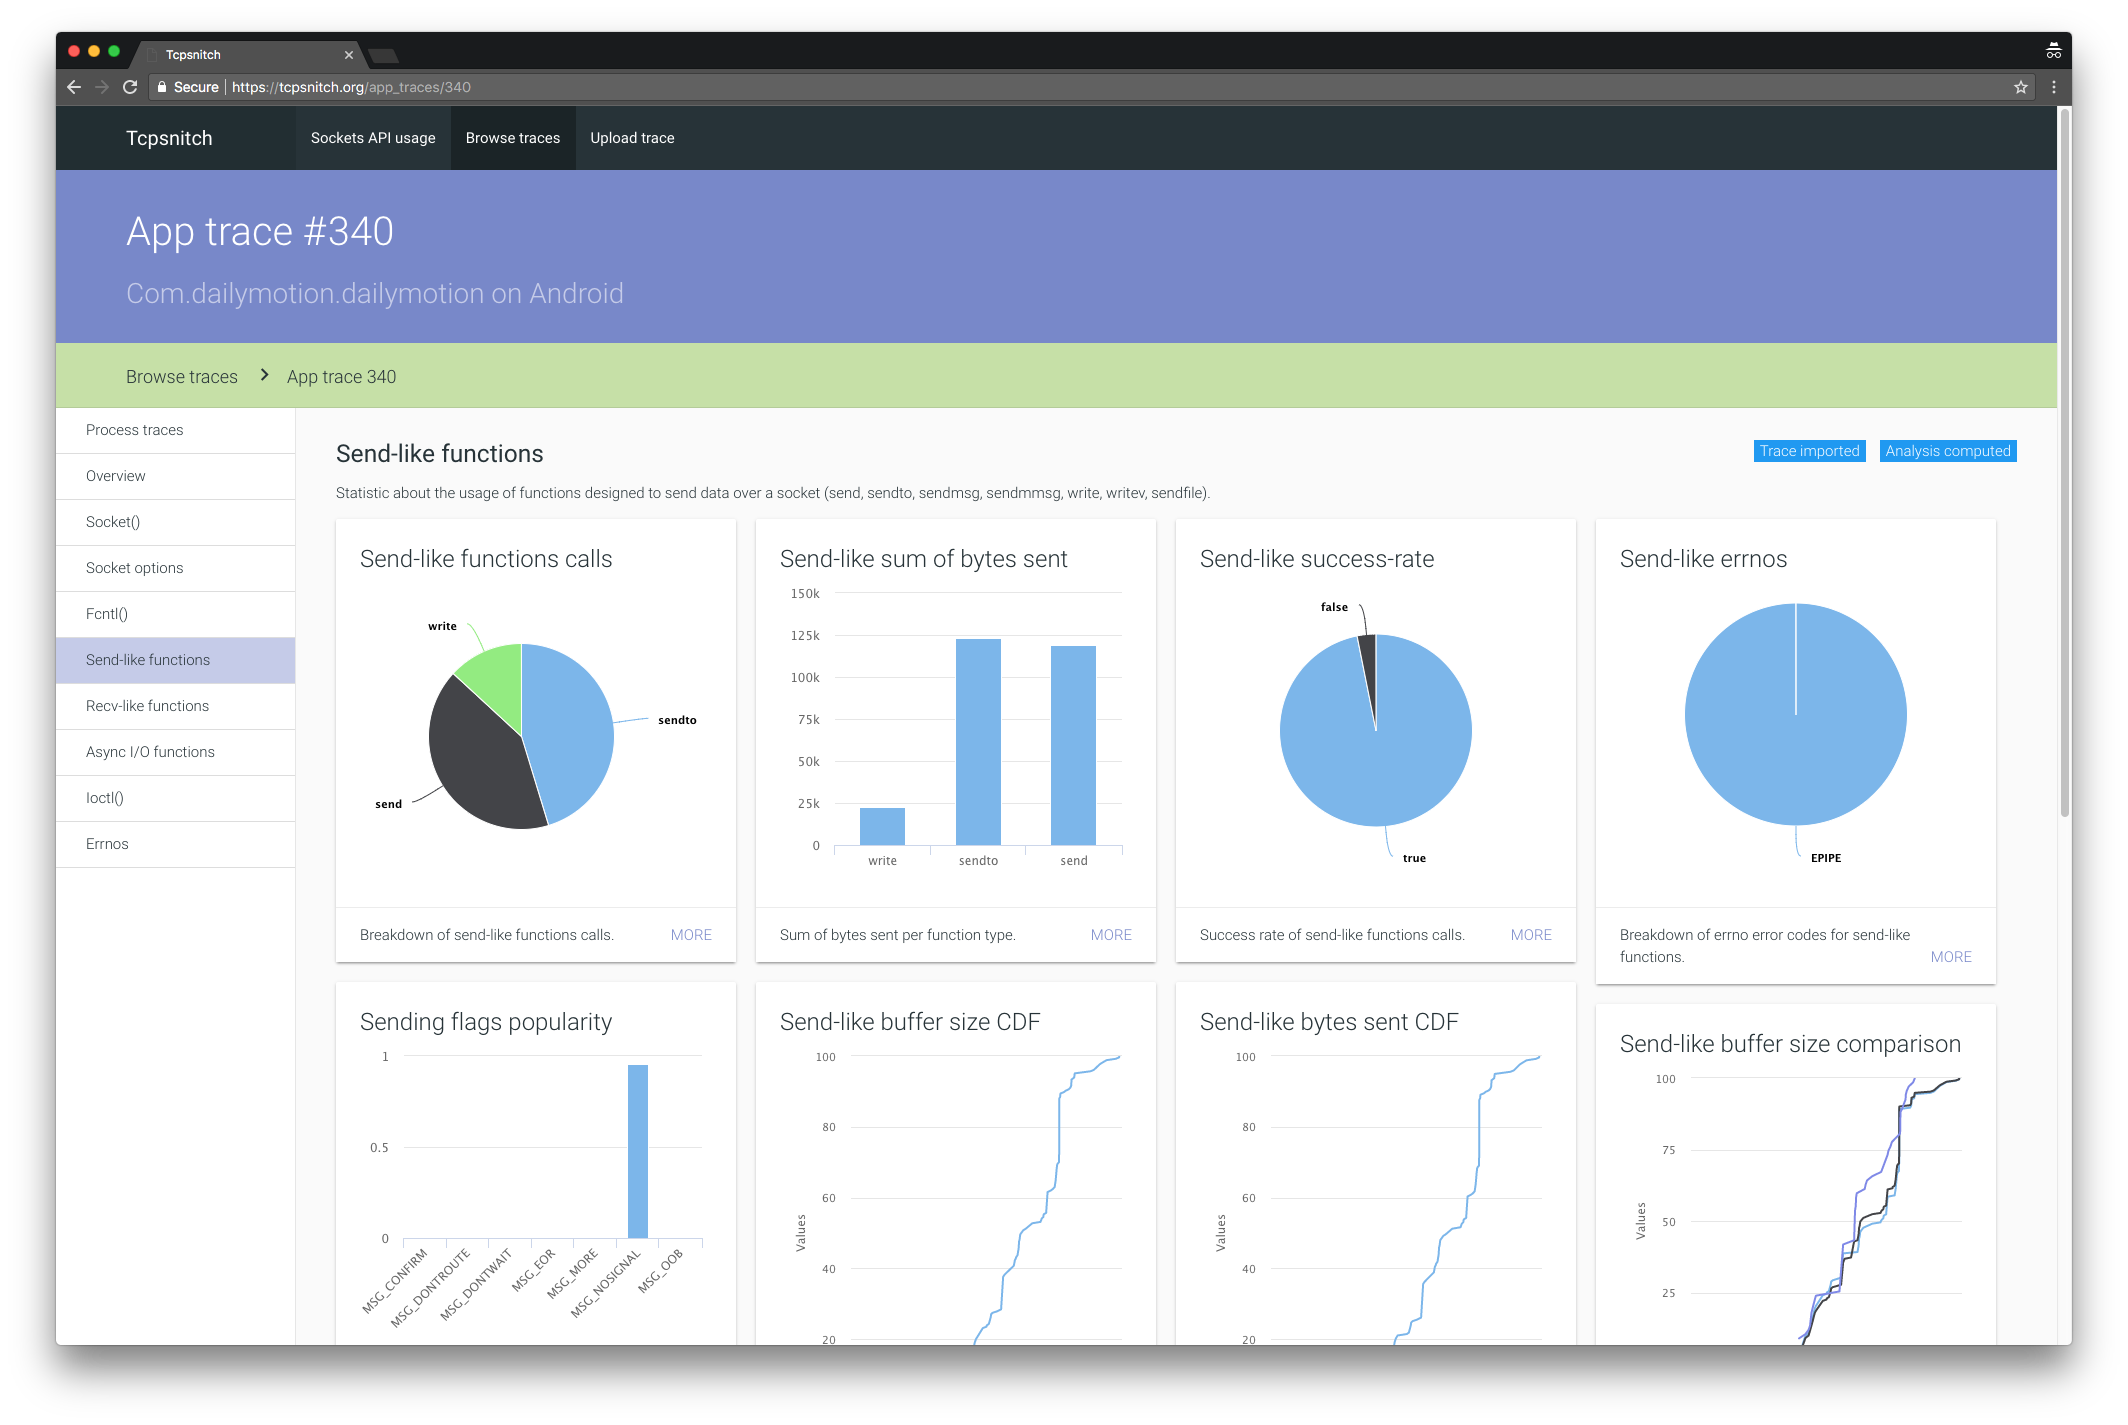
\includegraphics[width=.4\textwidth]{figures/org2}
        \end{tikzfigure}

        TCPSnitch.org is open-source: \url{https://github.com/GregoryVds/tcpsnitch_web}.
    }
\end{columns}



% THRID ROW
\begin{columns}
    \column{0.50}
    \block{API usage on Linux and Android differ greatly}{
        \begin{tikzfigure}
            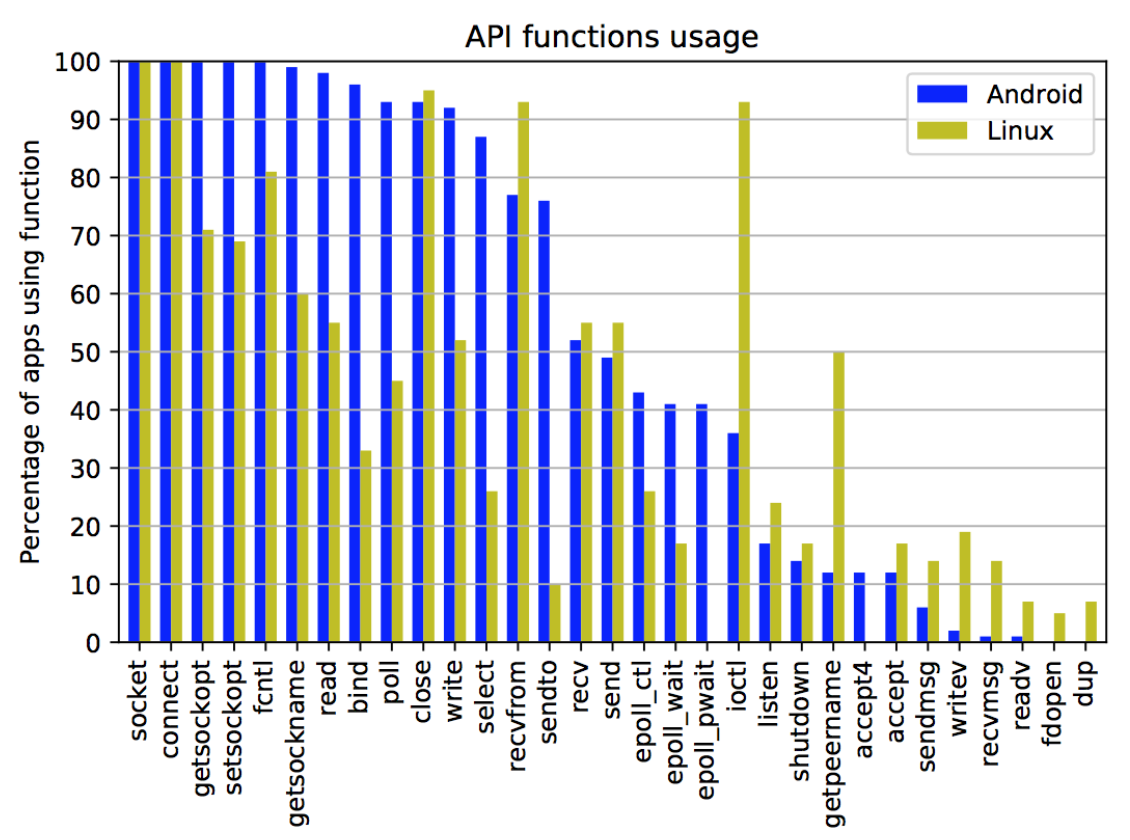
\includegraphics[width=0.40\textwidth]{charts/finding1}
        \end{tikzfigure}
    }
    \column{0.50}
    \block{API usage driven by high-level frameworks and libraries}{

    An HTTP GET request over TLS yields different API footprints with different libraries.\\
\begin{tikzfigure}
\begin{tabular}{lllllll}
\hline
\textbf{Language}   & Ruby        & Python   & JavaScript        & Perl        & PHP\\ \hline
\textbf{Library}        & \texttt{Net:HTTP} & \texttt{urllib2}  & \texttt{https mod}  & \texttt{LWP::Simple} & \texttt{f\_g\_contents} \\ \hline
\textbf{API calls}  & 186         & 353      & 106               & 465         & 920\\ \hline
\textbf{Bytes recv} & 65~KB       & 175~KB   & 175~KB            & 178~KB      & 175~KB\\ \hline
\textbf{Main API call}  & \texttt{read()}      & \texttt{read()}   & \texttt{read()} & \texttt{read()}      & \texttt{fcntl()} \\ \hline
\textbf{Socket option}  & \texttt{TCP\_NODELAY} & \texttt{SO\_TYPE} & \texttt{SO\_ERROR} & \texttt{SO\_ERROR} & \texttt{SO\_ERROR}\\ \hline
\textbf{Async I/O}      & \texttt{ppoll()} & N/A      & N/A  &  \texttt{select()} & \texttt{poll()} \\ \hline
\end{tabular}
\end{tikzfigure}

        \vspace{5cm}
    }
\end{columns}


% FOURTH ROW
\begin{columns}
    \column{0.33}
    \block{Android: API functions usage}{
        On Android, the API functions usage differs from textbook usage. Some
        unexpected functions are widely used.
        \begin{tikzfigure}
            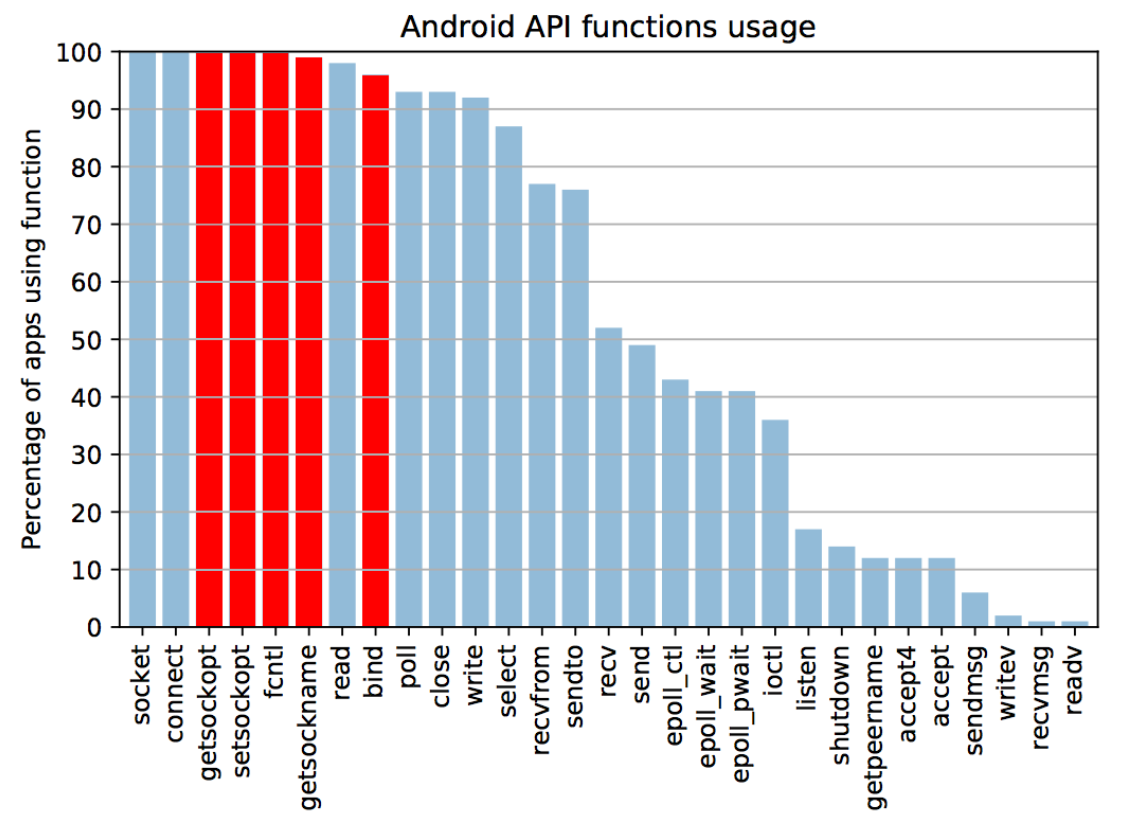
\includegraphics[width=0.25\textwidth]{charts/finding3}
        \end{tikzfigure}
    }
    \column{0.33}
    \block{Android: UDP sockets usage} {
        On Android, UDP sockets are mainly used as a shortcut to retrieve
        information about the network configuration.
        \begin{tikzfigure}
            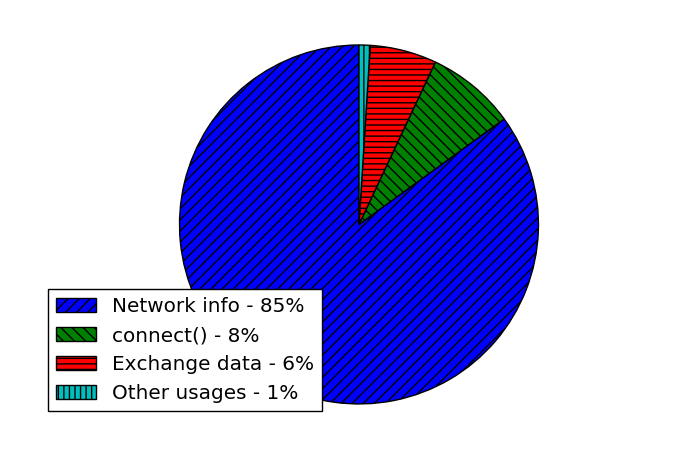
\includegraphics[width=0.27\textwidth]{charts/finding4}
        \end{tikzfigure}
    }
    \column{0.33}
    \block{Android: TCP\_INFO usage}{
        For some applications, the number of TCP\_INFO calls is a linear
        function of the number of recv() calls.
        \begin{tikzfigure}
           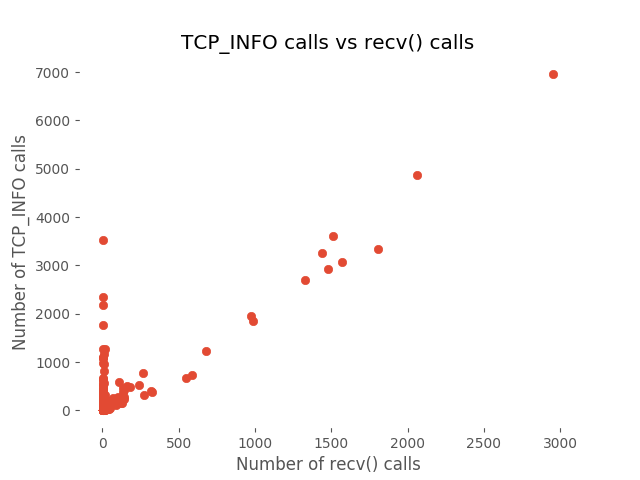
\includegraphics[width=0.25\textwidth]{charts/finding5}
        \end{tikzfigure}
%        \vspace{1cm}
    }
\end{columns}

\end{document}
